\subsection{Deployment}

I \textbf{deployment diagram} rappresentano la disposizione fisica dei componenti del sistema software nel contesto applicativo. Modello come insieme di \textit{nodi}.

\paragraph{Nodo} Contiene uno o più elaborati (\textit{artifact}): manifestazioni fisiche del sistema software (eseguibili, script di configurazione, librerie, jar, file di dati, documenti HTML, ecc...)

I nodi sono collegati da linee continue dette \textit{path} che forniscono informazioni sulla comunicazione tra essi (es. canale usato, protocollo adottato). I valori di etichetta (o \textit{tagged values}) specificano proprietà aggiuntive sui nodi.

\begin{figure}[H]
    \centering
    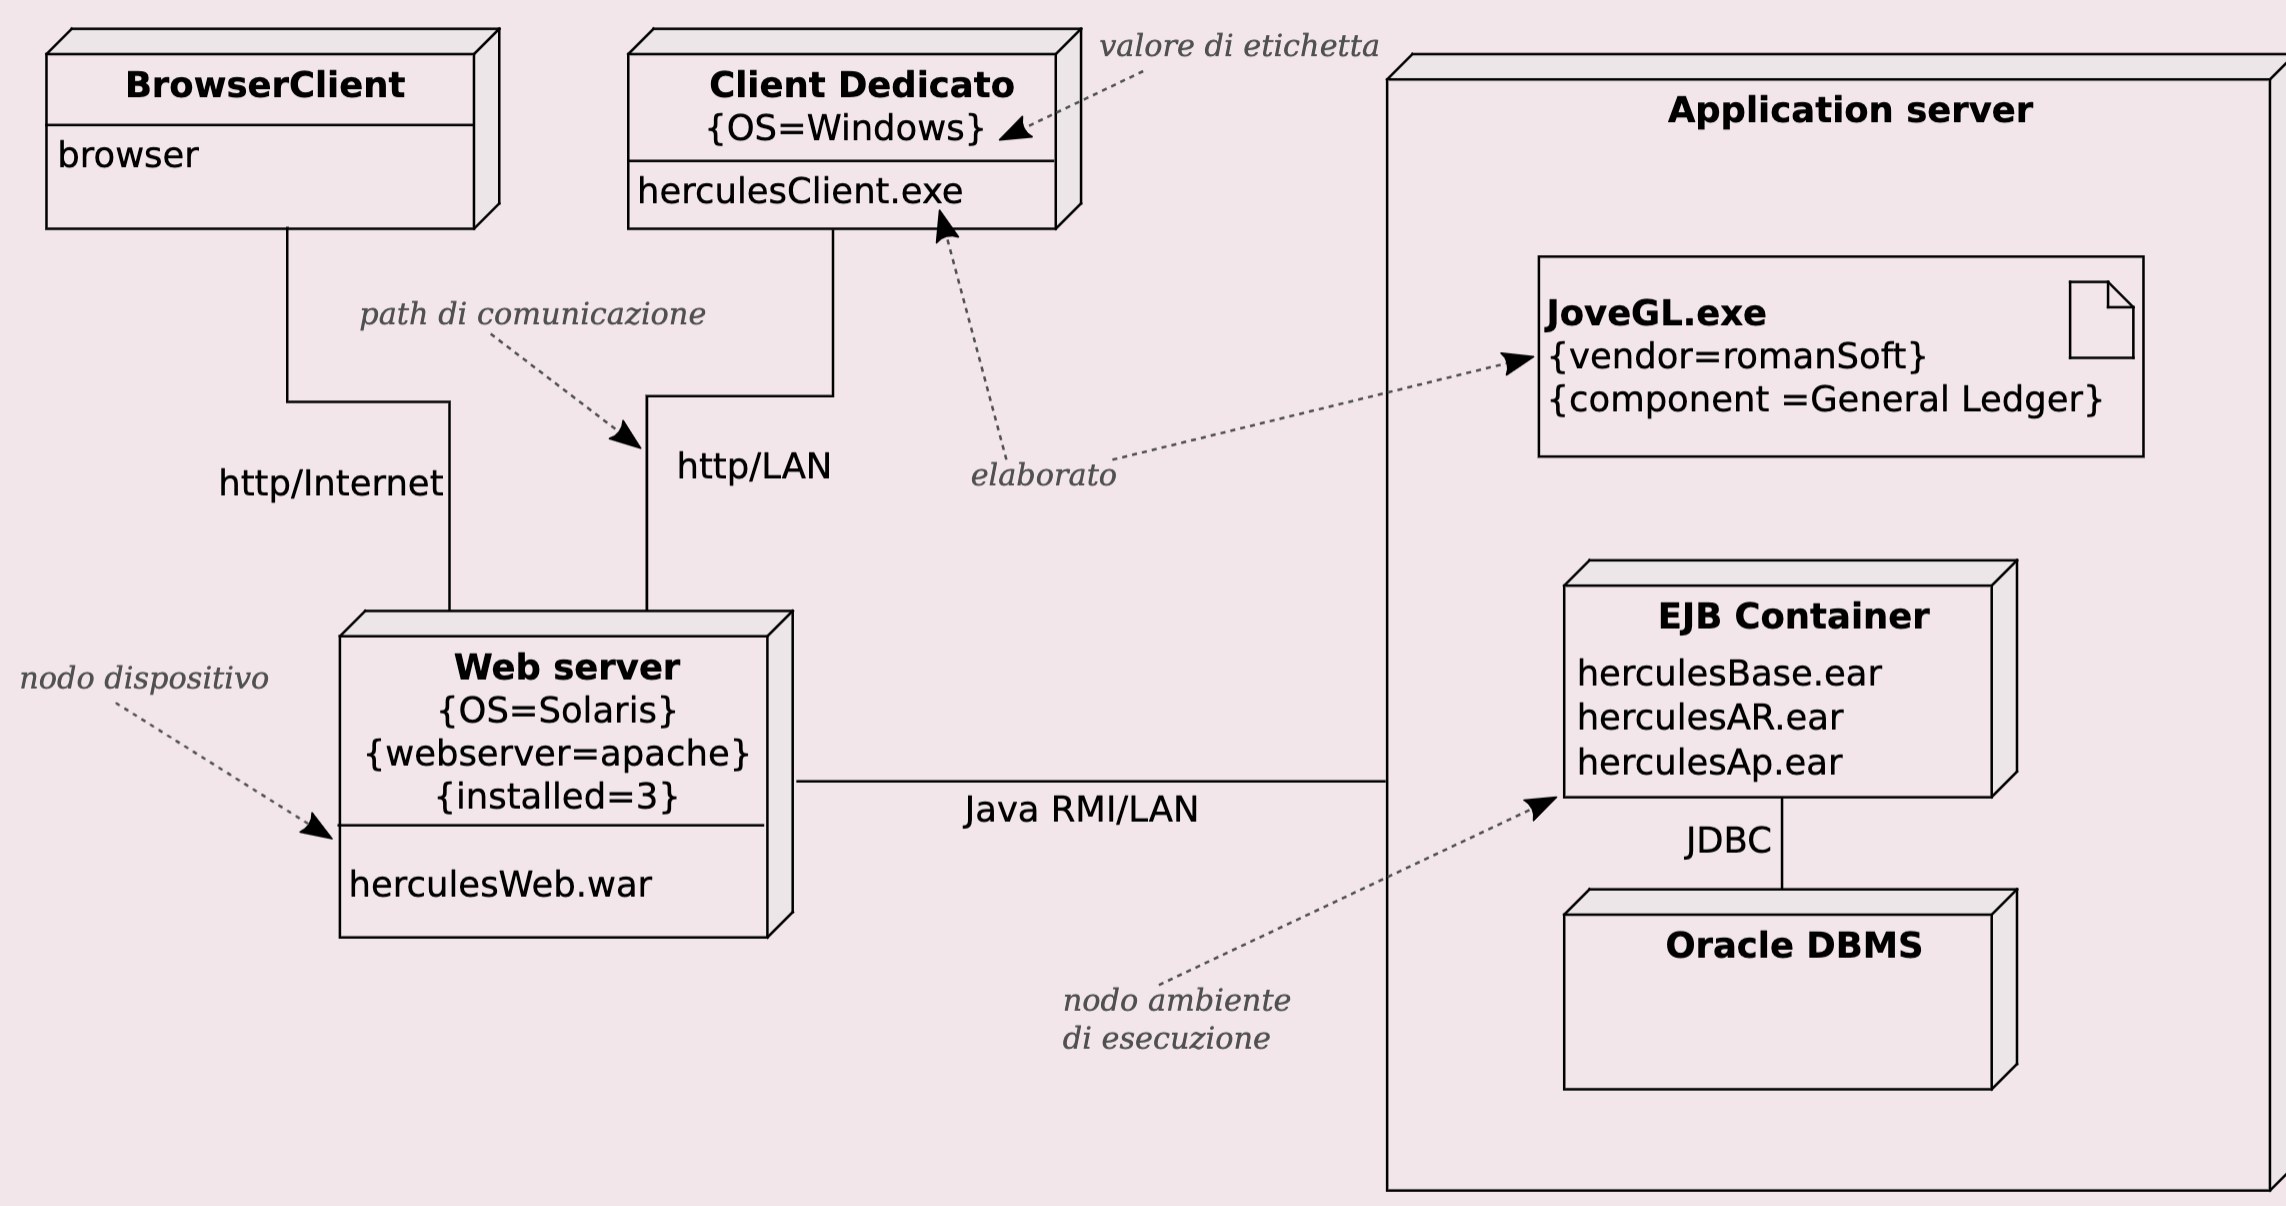
\includegraphics[width=0.75\linewidth]{assets/UML/deployment/deployment.png}
    \caption{Esempio di deployment diagram}
\end{figure}

\newpage